\documentclass[10pt]{article}
\usepackage{graphicx}
\usepackage[margin=1.5cm]{geometry}
\usepackage{amsmath}
\def\brcurs{{\mbox{$\resizebox{.16in}{.08in}{
\includegraphics{BoldR}}$}}}
\def\rcurs{{\mbox{$\resizebox{.16in}{.08in}{
\includegraphics{ScriptR}}$}}}

\begin{document}
\twocolumn

\title{Thursday Warm-up: Electrostatics}
\author{Prof. Jordan C. Hanson}

\maketitle

\section{Memory Bank}

\begin{itemize}
\item Gauss' Law, integral form
\begin{equation}
\oint \mathbf{E} \cdot d\mathbf{a} = \frac{1}{\epsilon_0}Q_{\rm enc}
\end{equation}
\item Gauss' Law, differential form
\begin{equation}
\nabla \cdot \mathbf{E} = \frac{1}{\epsilon_0}\rho
\end{equation}
\item Definition of potential
\begin{equation}
V(\mathbf{r}) = - \int_{\rm \mathcal{O}}^{\mathbf{r}} \mathbf{E}(\mathbf{r}') \cdot d\mathbf{l}'
\end{equation}
\item Relationship between potential and field:
\begin{equation}
\mathbf{E} = -\nabla V
\end{equation}
\item Electrostatic energy, point charges:
\begin{equation}
W = \frac{1}{2}\sum_{i=1}^n q_i V(\mathbf{r}_i)
\end{equation}
\item Electrostatic energy, continuous charge distribution:
\begin{equation}
W = \frac{1}{2}\epsilon_0\int E^2 d\tau
\end{equation}
\item Capacitance, $C$:
\begin{equation}
C = Q/V
\end{equation} 
\end{itemize}

\begin{figure}
\centering
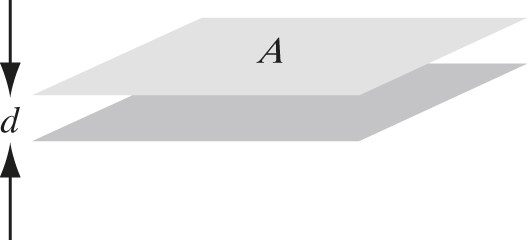
\includegraphics[width=0.2\textwidth]{figures/2_52.jpg}
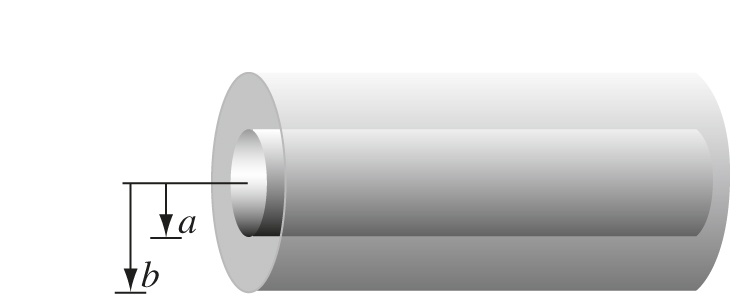
\includegraphics[width=0.25\textwidth]{figures/2_53.jpg}
\caption{\label{fig:1} (Left) A parallel-plate capacitor. (Right) A cylindrical coaxial cable with capacitance per unit length.}
\end{figure} \vspace{2cm}

\section{Gauss' Law and Scalar Potential}

\begin{enumerate}
\item Suppose the voltage (scalar potential) of a charge distribution obeys
\begin{equation}
V(\mathbf{r}) = A \frac{e^{-\lambda r}}{r}
\end{equation}
\noindent where $A$ and $\lambda$ are constants.  Find $\mathbf{E}(\mathbf{r})$, $\rho(r)$, and the total charge, $Q$. \\ \vspace{3cm}
\end{enumerate}

\section{Electrostatic Energy}

\begin{enumerate}
\item What is the electrostatic energy of an electric dipole, with a charge $+q$ at $(d/2)\hat{\mathbf{x}}$, and a charge $-q$ at $-(d/2)\hat{\mathbf{x}}$? \\ \vspace{1.5cm}
\end{enumerate}

\section{Capacitance}

\begin{enumerate}
\item Consider the conductors in Fig. \ref{fig:1} (Left). Show that the capacitance is $C = \epsilon_0 A/d$. \\ \vspace{2cm}
\item Consider the conductors in Fig. \ref{fig:1} (Right).  Show that the capacitance per unit length is $C/l = 2\pi\epsilon_0/\ln(b/a)$.
\end{enumerate}

\end{document}
